% vim: set fenc=utf-8 ft=latex encoding=utf-8
% -*- mode: latex; coding: UTF-8; -*-
%!TEX root = knowledge-curation.tex

\section{Discussion}
\label{cha:theory}

    In this section we present a theory that encapsulates the observations and insights found during the analysis of the data, including, the comparison of the
    way knowledge is shared on both channels, and the recommendations of the use of Q\&A communication channels.
    We also discuss them with respect to the related literature.

%Categorization of the way resources are used on Q\&A media channels.
\subsection{knowledge creation and curation}

    Based on our results, both channels provide roughly the same knowledge support for questions and answers.
    However, there are some differences between both channels which are summarized in Table~\ref{table:constrat}.
    These observations are tendencies, and they are not behaviours unique of each channel.

    \begin{table}[!htb]
      \centering
      \caption{Comparison of the way knowledge is shared on Stack Overflow and the R-help mailing list.}
      \label{table:constrat}
      \begin{small}
        \setlength{\tabcolsep}{5pt}
        \begin{tabular}{@{}lll@{}}
          \toprule
          \textbf{}      & \textbf{Stack Overflow} & \textbf{R-help}\\
          \midrule
          Knowledge construction & Crowd-based             & Participatory \\
          Topic restriction      & Yes & No \\
          Emphasis & Curating Knowledge & Developing Knowledge \\ 
          \bottomrule
        \end{tabular}
      \end{small}
    \end{table}

\subsubsection{Knowledge construction}

Stack Overflow's gamification system encourages being the first to answer the question~\cite{Singer2013}. In contrast, \RH is less competitive environment,
where users tend to build on other
responses; they work more as a team, rather than as individuals searching for points.
As 
a result, in \SO knowledge is built more in a crowd-source manner, while in \RH it is usually build in a participatory manner.

Even when the diversity of answers provided in Stack Overflow is high, users tend to not contribute (edit or comment) to such answers; instead, some users provide their own answers.
    For example, in the Stack Overflow thread \textit{``Resources for learning SAS if you already familiar with R''}\footnote{\url{http://goo.gl/Mb4Pbk}}, three of the six answerers referenced the same books.
%    The gamification mechanism gives reputation to those who answer the questions, even when each extra answer might not add any new insight about how to solve a specific problem.
    Stack Overflow curation mechanism is a powerful way to make sure the best answers make it to the top, but it does not provide a mechanism to explain why an
    answer is better than others.

    In contrast, the R-help mailing list tends to be more collaborative on how users construct knowledge, and discuss proposed answers. Its
    participants tend to provide more background to the answers and explain better the rational behind answers.

These differences are demonstrated in the question \textit{``Arrange elements on a matrix according to rowSums + short `apply' Q''}  posted to  Stack Overflow\footnote{\url{http://goo.gl/a8AES8}} and {R-help}\footnote{\url{http://goo.gl/PGflT5}}.
    Each communities answered the question using a different knowledge construction approach.
    On Stack Overflow, participants provided each their own solution without any evidence of collaboration between them.
    Whereas users on the R-help mailing list complemented each other answers by providing extra information and insights into the answers.
    
    The Stack Overflow's knowledge construction is not limited to crowd knowledge construction, it also presents collaborative ways to construct knowledge (such
    as voting up/down questions and providing comments).
    However, the crowd-based construction appears to be the more prevalent.
    Similarly, in \RH, knowledge is also crowed-constructed, but this form is less prevalent than the participatory one.

    Tausczik \textit{et al}.~\cite{Tausczik2014} found the same collaborative knowledge construction over another knowledge domain and channel, the mathematics domain on Math Overflow (a Q\&A channel focused on solving mathematical problems).
    Thus, we extend what Tausczik \textit{et al}. found to other communication channels and domains.

    Our results seem to imply that the gamification features of \SO, nonetheless effective, have the side effect of reducing collaboration between users towards knowledge creation.
    While \SO gives users the ability to vote on comments, it does not reward with points those who posted the comment\footnote{Some \SO \textsf{mercenaries}
      recommend searching for answers in comments and convert them to proper answers to gain reputation (e.g. \url{http://goo.gl/0qUjQw}).}.
    % The findings presented here as theory can be used to identify how channels' features or community members might affect the construction of knowledge.
    % For instance, we identified that gamification might affect collaboration between users. 
    % Users prefer to create their own answer instead of collaborating with others.
    % Additionally, it might be possible for indirect collaboration, like the one happening on the comments on Stack Overflow to improve discussion and participatory knowledge construction if there was a mechanism to provide points for this type of participation.
%    However, more studies are required to extend our observation to other domains, communities, and channels.

\subsubsection{Topic restriction}

The participation rules of \SO make it topic restrictive, since it only allows questions that have a clear answer; in contrast, the R-help mailing list is suitable to discuss
any topic regarding R. For example, on \RH, questions related to R, but not focused on software development, are not rejected by the community (see section
\ref{cha:findings-types} Flags).\dmg{give a concrete example?}
The study by Squire~\cite{Squire2015a} found a similar difference between Stack Overflow and a mailing list of multiple projects.

Topics that trigger a discussion are welcomed in to the R-help mailing list. 
%    For instance, when users discuss the creation or improvement of the R community channels (see section \ref{sec:userbeh}); or when a question about installing R on \textit{Linux} is asked on the R-help mailing list (like {\href{http://goo.gl/1JLOUF}{\textit{``R on X11 under Linux''}}}).
In contrast, in Stack Overflow questions that trigger a discussion are flagged as opinion-based, or as off-topic, and they are likely to be closed. 
For example, the questions \textit{``What's a good example of really clean and clear [R] code, for pedagogical purposes?''}\footnote{http://goo.gl/9JjZW1} was
closed as off-topic because the question was not related to software development. 
The advantages of each channel are explained by a user in a message in \RH \emph{``creating an equivalent of r-help on r.stackexchange.com?''}\footnote{\url{http://goo.gl/mTccwx}}:
    \begin{quote}
        \textit{``got an R programming question that you think has a definite answer? Post to [Stack Overflow]. Want to ask something for discussion, like what options there are for doing XYZ in R, or why lm() is faster than glm(), or why are these two numbers not equal-- post to R-help. Questions like that do get posted to [Stack Overflow], but we [moderated] them down for being off-topic and they disappear pretty quickly.''}
    \end{quote}

    % We believe it is important to understand how the knowledge is constructed on media different channels, and how different mechanisms such as gamification or topic restriction can affect the knowledge construction~\cite{Li2015}.
    % Through this understanding, researchers can gain insights of how to support future media channels, and user diversity~\cite{Vasilescu2014b}.

\subsubsection{Curated knowledge and knowledge development}

    The main benefit of using crowd-based knowledge construction is the creation and maintenance of a pool of questions and answers. In contrast, \RH provides an environment in which users
    develop knowledge through participation, but this knowledge is not curated for future use, making it difficult to be reused by those who were not
    participants (either active or passive) during its creation.


    % On the R-help mailing list questions tend to have more background than on Stack Overflow.
    % The knowledge embedded in the R-help mailing list's answers can be used to learn new procedures, as well as identify the train of thought that guided
    % participants when forming an answe
While \SO  has been successful, some users feel that by now fostering discussion, it restricts thinking that might lead towards better anwers. 
For instance, U26 explains:
    \begin{quote}
        \textit{``Many developers share my view that [Stack Overflow] is a very bad model, ... [it] removes the value added by reading list traffic that doesn't seem directly relevant to a currently conceptualised question, but which may lead to a new conceptualisation (out of the frame thinking). [Stack Overflow] cannot do that.''}
    \end{quote}
    Similarly, U35 explains that it uses the R-help mailing list if the questions are not 100\% \textit{``help-me-to-code-this''}.

    In contrast, Stack Overflow shines when questions have to be kept for posterity. 
    The curation mechanism provides tools to keep the channel clean of what seems to be unnecessary information (e.g., flagging questions, deleting comments, editing messages, and demoting irrelevant answers).

    \begin{quote}
        \textit{``[Stack Overflow] is an excellent model for providing a rich resource for users of R, which the R-Help mailing list was not. 
        Ability to include light markup, render code blocks nicely, [and] not [having] nested email threads all helps the experience of searching for and finding the help that a user needs, and I want to contribute to that.''} [U14]
    \end{quote}

    % Thus, we identified that there are certain benefits for keeping the history of the question available.
    % As U26 said, there are some benefits to reading what a user thinks is not important for conceptualized questions, but which may lead to out of the frame thinking. 

An important research question that arises from these findings is whether \SO can be improved with a more participatory development of knowledge without
hindering its ability to curate it for future use.


\subsection{Recommendations for using multiple Q\&A communication channels}

    One of the expected outcomes of this study was to derive a set of recommendations for using different communication channels.
    % Based on the analysis of the \textit{flags} (which are often used to point out users' behaviours); rules, manuals and FAQ resources from Stack Overflow and the R-help mailing list; threads that were posted in both channels (i.e., the same question by the same user in both channels); and the answers of the survey.
    Based on our results, we provide four recommendations.

    By studying communities that migrated development support towards Stack Overflow, Squire~\cite{Squire2015a} found that the main reason for communities coming back to the mailing list are topic restriction and the question's format expected on Stack Overflow.
    Squire and us suggest that communities of practice should evaluate the real benefits of each channel before moving to newer technologies.


    \begin{table*}[htbp]
      \caption{Recommendations to improve the benefits from using several Q\&A communication channels.}
      \centering
\small
      \begin{tabularx}{1.0\linewidth}[h]{p{4.6cm}p{12.5cm}}
\reca & Make sure the channel is the best according to the specifics of the question.\\
\recb & Make sure the question uses the proper nomenclature and does not violate the rules of the channel.\\
\recc & Explain the context that prompts to ask the question.\\
\recd & Reference external resources appropriately and use tools (such as gists.github.com) that make it easier for others to help.\\
\rece & Help others and work towards improving the community and the channels.\\
      \end{tabularx}
      \label{tab:recom}
    \end{table*}

\subsubsection{\reca}


    As described in section~\ref{cha:background}, each channel provides a list of \textit{topics} that are deemed acceptable.
    The control of topics is regulated either by the community or channel's moderators.
    U35 explains that \textit{``...Stack Overflow has more limited range of help topics (help for code only), whereas R-help is broader (philosophy, posting announcements, etc.)''}.
    \textbf{Knowing what channel is more suitable for a specific topic can improve the response time or quality of the answer}.

\dmg{The following is not clear and I would delete it}
    Additionally, \textbf{choosing the proper channel keeps the knowledge where it is most useful, thus enhancing the quality of the content of the channel}.
    For example, in the R-help's thread \textit{``Bumps chart in R''}\footnote{\url{http://goo.gl/EJHWrs}}, a user wrote: \textit{``(cross posting to the ggplot2 group for posterity) Here's how I'd approach it...''}, that is, cross-posting the question---previously posted and answered on the R-help list---in order to keep a record of the knowledge where it reaches more users, and where it is more useful to the community.

    In some cases, questions are expected to be \textbf{answered by a \textit{specific group} (e.g., r-core team) regardless of the topic}.
    U32 stated \textit{``If I really want an answer from someone in R-core or closely related people, I would definitely choose the mailing list''}.
    For example, in the R-help's thread \textit{``Cointegration and ECM in Package \{urca\}''}\footnote{\href{http://goo.gl/7olLv7}}, a participant asked the R-core team directly how to solve a problem: \textit{``Dear R Core Team, I am using package \{urca\} to do cointegration and estimate ECM model, but I have the following two problems...''}.
    In this scenario, \textbf{websites of a specific package or library might be the best method to communicate directly with the creators of that technology}.
     

\dmg{I do not understand the following}
In some cases, the description of the channel or package provides the necessary information, such as the maintainers or participants (e.g., R-help primary help webpage\footnote{\url{https://stat.ethz.ch/mailman/listinfo/r-help}}, \emph{rcpp} package\footnote{\url{https://cran.r-project.org/web/packages/Rcpp/index.html}}, or \textit{r-tag} info page on Stack Overflow\footnote{\url{http://stackoverflow.com/tags/r/info}}).
    Figure \ref{fig:CCchannel} depicts an example of how developers of a package can be reached using Stack Overflow (on the left) or by email (on the right). 

    \begin{figure} [!htb]
        \centering
        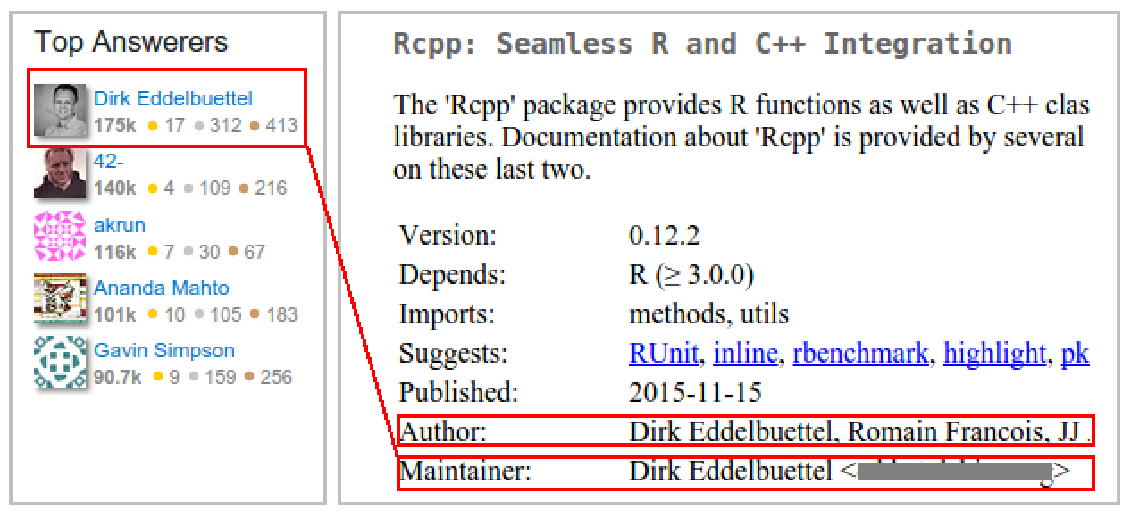
\includegraphics[width=\columnwidth]{Figures/CCchannel}
        \caption{Example of how to reach developers of the \emph{rcpp} package. On the left, Stack Overflow, and on the right, the \emph{rcpp} webiste.}
        \label{fig:CCchannel}
    \end{figure}

%    Some channels are more suitable for certain \emph{type or format of questions}. 

Thus, R-help is a place for discussion, and Stack Overflow is a place for questions that have a clear answer.


\subsubsection{\recb}

    Throughout this study, we noticed that most of the harsh responses were given to users who did not read the posting guide or had learned the basic concept of
    R or statistics.
    The community expects that if someone wants to use a channel, they should learn about it in advance, and learn the basics of the technology that they are using.

    % For instance, in the R-help's thread \textit{\href{http://goo.gl/Dc8gXw}{``Quantile''}} it is remarked the points of a guide that the user asking the question did not follow: \textit{``...Please read the Posting Guide. It asks that you not crosspost. If you post a followup to rhelp, then the reading of the Posting guide will tell you that much more in the way of detail about your setup was requested...''}.

%    Depending on the channel, the amount of guide lines and posting guides available might differ. 
    Stack Overflow provides user manuals\footnote{\url{http://stackoverflow.com/help}} for each of the main features of the channel, such as badges, questions,
    answers, flags, comments, and reputation system.     In contrast, \RH only has general instructions\footnote{\url{https://www.r-project.org/mail.html\#instructions}} and the posting guide user manual\footnote{\url{https://www.r-project.org/posting-guide.html}}.

    Moreover, depending on the purposes of the communication channels, there might exist community-developed guide that should be read before participating in the channel.
    For example, the post on Stack Overflow \textit{``How to make a great R reproducible example?''}\footnote{\url{http://stackoverflow.com/questions/5963269/how-to-make-a-great-r-reproducible-example}} provides tips and tricks for creating a reproducible example using the R language.
    Another example is the guide for \RH written by Hadley Wickham \emph{How to write a reproducible
      example}\footnote{\url{http://adv-r.had.co.nz/Reproducibility.html}}, geared towards mailing lists. 
    It provides tips for posting R to mailing lists, such as: \textit{``...Before putting all of your code in an email, consider putting it on \url{http://gist.github.com/}{[GitHub Gist app]}. It will give your code nice syntax highlighting, and you don't have to worry about anything getting mangled by the email system...''}

    Finally, there are manuals like \textit{``An Introduction to R''}), and the FAQ webpages that are available to the public---most of the time free of charge,
    from which any user can learn the basic of each technology.
    For example, the R community provides a compendium of PDF documents for new users on different languages\footnote{The R Manuals are available at \url{https://cran.r-project.org/}}.
    In Stack Overflow, supported technologies are provisioned with webpages and links to free and paid materials\footnote{Materials available at \url{http://stackoverflow.com/tags/r/info}}.
    %Members are able to reference these materials when needed, e.g., \textit{``...You may want to acquaint yourself with the 'An Introduction to R' manual that came with your R installation to learn more about indexing.''}



\subsubsection{\recc}

    In spite of reading the documentation available, a user may fail to address the channel appropriately.
    The community may feel that the question asked, the information provided or something else is not in compliance with the expectations and rules of the channel.
    In such cases, one should describe the documentation read, the attempts made, and what is being trying to achieve.
    This would avoid answers like \textit{``read the manual''} or \textit{``read the posting guide''}, as well as helping the participants to help.
    As an example, in the thread \textit{``lme4 GLMM''}\footnote{\url{https://goo.gl/Gbek3R}}, the user explicitly acknowledged the repeated question, and
    explained his rational for doing so: \textit{``I'm very sorry for my repeated question, which I asked 2 weeks ago, namely: I'm interested in possibly simple random-part specification in the call...''}.


\subsubsection{\recd}

    A common practice to answer or ask questions is to provide links for documentation, examples, source code, or other resources.
    As links point to online resources that might not exist in the future, it is important to include the key points of the resource within the question or answer.
    For instance, when a question or answer contains information in an external file hosting service like Dropbox or Google Drive, the owner of the service account can break the link at any moment, leaving the message incomplete or impossible to reproduce, like the thread \textit{\href{http://goo.gl/5nanFU}{``Is it possible to create a 3d contour plot without continuous data in R?''}}.
    U33 suggested: \textit{``Questions should be self-contained as much as possible. Exceptions: recognizable links such as CRAN, R documentation, etc.''}.

    Based on our observations, we constructed a set of recommendations for links that are the exception of the rule:

    \begin{description}[itemsep=3pt, topsep=2pt, leftmargin=3em, parsep=0pt]
        \item[Well known websites] are expected to be maintained in the long term like Wikipedia, the official documentation in CRAN.
        For example, the Stack Overflow's thread \textit{``calculating convolution of multinomial distribution''} a user posted \textit{`I'm doing a simulation where I need to calculate a \href{https://en.wikipedia.org/wiki/Convolution_of_probability_distributions}{[Wikipedia convolution]} of \href{https://en.wikipedia.org/wiki/Multinomial_distribution}{[Wikipedia multinomial distributions]}...''}.

        \item[Resources that support or expand the message] when the important information is already in the message.
        For instance, the Stack Overflow's thread \textit{``How do I save all the draws from a MCMC posterior distribution to a file in R''} clarifies \textit{``...You should be able to open a text connection using ?file \href{http://stat.ethz.ch/R-manual/R-devel/library/base/html/connections.html}{[more information]} with the open argument set to write...''}.

        \item[Material relevant to the message is too big] as papers or demonstrations.
        For instance, the R-help's thread \textit{``Using FUNCTION to create usable objects''} a user stated \textit{``I suspect you are trying to find your way into Circle 6 of 'The R Inferno' but haven't yet got in. \href{http://www.burns-stat.com/pages/Tutor/R\_inferno.pdf}{[R Inferno]}''}.
    \end{description}

\subsubsection{\rece}
\label{sec:userbeh}

It is obvious that users help others by answering questions. However, while analysing questions and answers, we identified positive user behaviours that
we believe are worth mentioning.  These behaviours provide evidence of their altruistic way of thinking and the strong commitment that users have within their
community towards knowledge building.

\begin{packed_enum}
\item \textbf{I answered my own question}: Some questions are answered by the same user who asked the question. They posted back to the channel to document
  their solution and help others.
        For example, \textit{``I've discovered the answer to my own question.''}\footnote{\url{http://goo.gl/FG59Mw}} or \textit{``Just for the records (and if
          anyone ever wants to find the `solution'), I solved my own problem.''}\footnote{\url{https://goo.gl/r3z0DX}}. 
 
        \item \textbf{I did it for you}: When answering, authors provide source code to help others. For example, \textit{``I have coded up the algorithm from the Cameron and Turner paper. Dunno if it gives exactly the same results as my (Splus?) code from lo these many years ago...''}\footnote{\url{http://goo.gl/GXWGG3}}.

        \item \textbf{Updated or continued years later}: Some answers are provided months or years after the question was asked.
        For example, a user on Stack Overflow modified an answer to provide a more updated version of the source code\footnote{\url{http://goo.gl/k6ZARR}}; and a {question asked on the R-help mailing list in 2012 was continued two years later}\footnote{\url{http://goo.gl/kgSHZv}}.

        \item \textbf{Ideas for improvement or creation of the channel}: This behaviour is specific for the R-help mailing list. Sometimes users suggest modifications or new features to improve the channel. For example, a {user proposes to create a package repository that can be accessible through a public wiki, or version control interface}\footnote{\url{http://goo.gl/p0IunD}}.
    \end{packed_enum}

% \dmg{I would remove the two following bullets:}

%     We also identified 2 behaviours that might result in a negative response from the community:
%     \begin{packed_enum}
%         \item \textbf{Cross-posting:} The user posts the same question in both channels at the same time.
%         For instance: \textit{\href{http://goo.gl/ENKrVK}{``-1 for cross posting to r-help – [user name]''}}.
% \dmg{This needs an example of a bad response, not just a crossposting, since this example does not show why users dislike it}
% \dmg{This next one sounds repetitive... it is already above in learn to use the chnanel}
%         \item \textbf{Posting guidelines violation:} The user behaves in a way that it becomes apparent that they did not read the posting guidelines.
%         For instance, a user asked a question that seems to be the opposite of what the posting guide recommend, and someone answered: \textit{\href{http://goo.gl/FUm1HC}{``...If you read the Posting Guide I think you will find precisely the opposite expectation explicitly presented. Using my "cheeky code" would only be part of the recommended actions to take before posting if you follow the recommendations of the "Do your homework before posting:"...''}}.
%     \end{packed_enum}



\section{Threats to validity}
\label{cha:threats}

\remarks{Consider make the data available online.}

Regarding construct validity: the open coding of a large collection of messages may introduce bias.  To minimize this thread we used multiple data sources to
triangulate our findings (survey, documentation, and messages from two different communication channels), we randomly selected data, and two researchers
performed the data coding. We applied the Cohen Kappa coefficient on categories that were not mutually exclusive, whose purpose was to trigger discussion
between coders.  We set a threshold of 80\% as the minimum to obtain agreeable results, which is higher than the 60\% suggested in the
literature~\cite{Landis1977}. 

Regarding internal validity: in order to compare the emails to the stack overflow discussions we had to map the types of messages from one channel to the
other. The R-help mailing list is unstructured emails that are connected between each other when they belong to the same thread. In contrast, \SO has a rich
data type (questions, answers, comments, flags, etc.). Some of this mapping is automatic: a reply is a response to the original question, a follow-up to a reply
is a comment to that question. Other had to be done by hand, this includes identifying some emails as containing a question, or a being a ``flag''.
Also, \SO is newer than \RH, and for that reason we only used messages from \RH that were created after \SO was created.
Two researchers performed this mapping to reduce any bias that it might have  introduced.

% Additionally, our understanding of that data and the observations we made played a big role in the mapping exercise, and it is subject to research bias.  To
% minimized the bias, two researches performed the mapping.

Regarding external validity: the nature of this study is to be exploratory and its findings only apply to the R community.
This type of case study cannot be assumed to be generalizable until further evaluations have been conducted~\cite{Yin2009}.
    Hence, the findings of this research should be tested in other communities and with other channels to see if they apply to these other contexts.
Another aspect to consider is that the R-community might not be composed of traditional programmers.
    The R programming language is used to solve statistical problems, where the product is the statistical analysis or graphs it creates. The scripts written in
    R are not the product, but the means to a product.
    Also, many R language users are likely to be \textit{casual developers} with limited or non-existent programming experience, with backgrounds that vary from
    biologists to statisticians. As a consequence, this study might not represent the knowledge that a software developer community shares. 

%%% Local Variables:
%%% mode: latex
%%% TeX-master: "knowledge-curation.tex"
%%% End:
